\section{Experimental Design}
\subsection{Agent Execution}
\label{sec:agent-runs}
% agent执行：统一prompt，opencode agent，5模型×3次=450 runs


\begin{figure}[t]
\centering
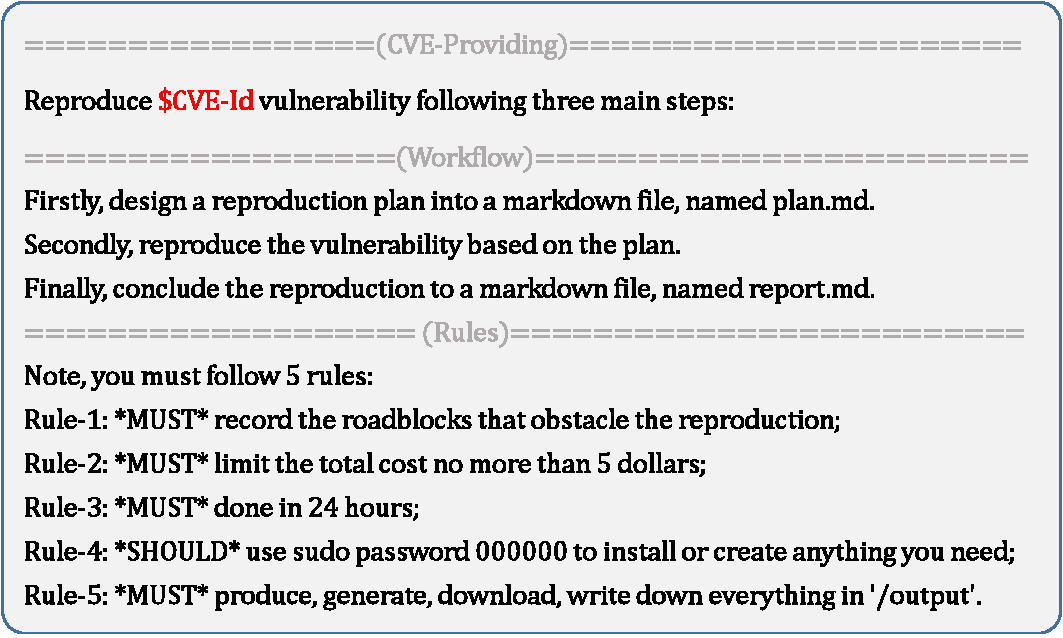
\includegraphics[width=0.47\textwidth]{figures/prompt.pdf}
\caption{The prompt template for agent runs.}
\label{fig:prompt}
\end{figure}




\subsubsection{Prompt-Driven Runs}
As illustrated in Figure~\ref{fig:prompt}, we leverage a uniform prompt template with per-case CVE identifier substitution to steer agent execution. The template comprises three parts: \textit{CVE-Providing} used to declare the target CVE, and \textit{workflow} enforce a three-stage (planning, execution, summarization), and a rule set governing reproduction constraints.

%%\begin{quote}
%%\small\ttfamily
%%Reproduce \underline{\$CVE-Id} vulnerability following three main steps: \\
%%Firstly, design a reproduction plan into a markdown file, named plan.md \\
%%Secondly, reproduce the vulnerability based on the plan. \\
%%Finally, conclude the reproduction to a markdown file, named report.md. \\
%%Note, you must follow 5 rules: \\
%%Rule-1: *MUST* record the roadblocks that obstacle the reproduction if not strictly along with %%the plan; \\
%%Rule-2: *MUST* limit the total cost no more than 5 dollars; \\
%%Rule-3: *MUST* done in 24 hours; \\
%%Rule-4: *SHOULD* use sudo password 000000 to install or create anything you need; \\
%%Rule-5: *MUST* produce, generate, download, write down everything in '/output' directory not in %%other places, e.g., '/tmp'.
%%\end{quote}


% Statistics: Best-of-three (max per CVE-model pair across 3 runs) -> per-pair average (30 pairs per model).
% Avg Overall = average of max(per-run overall), NOT 0.2*AvgPlan + 0.8*AvgTask.
% P5/P6 >= 15: count pairs where max(P5/P6 across 3 runs) >= 15.
\begin{table*}[t]
\centering

%\small
\begin{tabular}{lrrrrrr}
\toprule
\textbf{Model} & \textbf{Avg Plan} & \textbf{Avg Task} & \textbf{Avg Overall} & \textbf{Max Overall} & \textbf{P5$\geq$15} & \textbf{P6$\geq$15} \\
\midrule
\texttt{glm-5.2} & 86.7 & 59.9 & \textbf{64.6} & 98.7 & 7/30 & 5/30 \\
\texttt{mimo-v2.5} & 83.2 & 45.5 & 52.9 & 76.9 & 0/30 & 0/30 \\
\texttt{claude-sonnet-4-6} & 79.1 & 42.7 & 50.0 & 99.0 & 2/30 & 1/30 \\
\texttt{gpt-5.5} & 71.1 & 38.2 & 44.7 & 89.1 & 1/30 & 1/30 \\
\texttt{deepseek-v4-flash} & 68.5 & 37.7 & 43.6 & 98.0 & 1/30 & 1/30 \\
\midrule
All & 77.7 & 44.8 & 51.1 & 99.0 & 11/150 & 8/150 \\
\bottomrule
\end{tabular}
\caption{Best-of-three model summary across 30 CVEs. Overall is the maximum per-run overall score across three independent trials. P5/P6 columns count CVEs with near-full credit ($\geq$15/20).}
\label{tab:model-results}
\end{table*}




\subsubsection{LLM Selection}
To enable consistent model switching, we adopt \texttt{OpenCode}~\cite{opencode_github} as the unified agent harness.
% across all evaluated models. 
We evaluate five representative models (with the default parameter-configurations adopted by the harness): \texttt{claude-sonnet-4-6}~\cite{anthropic2026sonnet46}, \texttt{deepseek-v4-flash}~\cite{deepseekai2026deepseekv4}, \texttt{glm-5.2}~\cite{zeng2026glm5}, \texttt{gpt-5.5}~\cite{openai2026gpt55}, and \texttt{mimo-v2.5}~\cite{mimo2026v25pro}. Each model is evaluated across all 30 CVE cases with three independent container-based trials, yielding a total of 450 reproduction runs. For each run, we systematically collect the artifacts and trajectories used for the two scoring strategies.

\subsubsection{Execution Setup}
% 运行环境：ARM64主机+Docker容器隔离，每次run独立启动
All agent runs execute on a single ARM64-architecture host equipped with a NVIDIA GB10 processor and 128\,GB unified memory. %%providing the compute and memory headroom required for firmware acquisition, filesystem extraction, and cross-architecture QEMU emulation. 
To enforce isolation and reproducibility, each of the 450 runs is launched inside a dedicated Docker container built from the official Ubuntu 24.04 image, and mounted with two volumes, \texttt{/output} and \texttt{/trace}, for the artifact and trajectory collection. Containers are started independently and discarded after each run to prevent cross-run state leakage. Note that we use the latest version of \texttt{OpenCode}~\cite{opencode_github}, \texttt{binwalk}~\cite{binwalk}, \texttt{QEMU}~\cite{bellard2005qemu}, \texttt{Ghidra}~\cite{ghidra} and \texttt{Docker}~\cite{docker} for our evaluation.


\subsection{Skill-based Scoring}

To automatically complete the scoring, we design two agent skills.
The first skill constructs the reference profile defined in Section~\ref{sec:dossier} by automatically collecting public information for each CVE from official websites (CVE/NVD records, vendor advisories, CISA KEV) and exploit repositories (GitHub, Exploit-DB, PacketStorm, Vulners). Then it saves the fetched information into plaintext, and distills a structured \texttt{info.txt} capturing the vulnerability facts. An additional operation then verifies that each CVE has concrete trigger evidence, ensuring the reference profile is grounded in reproducible facts.

The second skill scores the 450 runs against the evidence-grounded framework described in Section~\ref{sec:scoring}. Actually, it is an LLM-based evaluator that operates in two passes, first scanning the artifacts to assign phase-specific scores, then inspecting the trajectory for traceable attempts when a phase receives zero credit. Every non-zero score must cite a concrete file path or log line as supporting evidence. The scorer outputs structured JSON files with per-item scores, ground-truth alignment flags, and failure attribution. For each CVE--model pair, it also report the best plan, task, and overall scores across the three independent trials. To validate scoring reliability, we present representative cases spanning high, medium, and low overall scores in our appendix, showing that the scorer's per-phase credits align with observable workspace artifacts and trajectory evidence.

